% This is samplepaper.tex, a sample chapter demonstrating the
% LLNCS macro package for Springer Computer Science proceedings;
% Version 2.20 of 2017/10/04
%
\documentclass[runningheads]{llncs}
%
\usepackage{graphicx}
\usepackage{listings}
\usepackage{amsmath,amssymb}
% Used for displaying a sample figure. If possible, figure files should
% be included in EPS format.
%
% If you use the hyperref package, please uncomment the following line
% to display URLs in blue roman font according to Springer's eBook style:
% \renewcommand\UrlFont{\color{blue}\rmfamily}

\lstdefinestyle{agree} 
 {frame=none, 
   basicstyle=\ttfamily, 
   language=ML, 
   aboveskip=3mm, 
   belowskip=3mm, 
   showstringspaces=false, 
   columns=flexible, 
   numbers=none, 
   numberstyle=\tiny\color{gray}, 
   commentstyle=\color{dkgreen}, 
   stringstyle=\color{mauve}, 
   breaklines=false, 
   breakatwhitespace=true, 
   tabsize=2, 
   linewidth=2\linewidth, 
   morecomment=[l]{--}, 
   escapeinside={*}{*}, 
   morekeywords={node, assume, eq, bool, guarantee, assume, true, false, pre, not, and, or, property, const, Historically, Since, Once, event, annex, Implementation, process, subcomponents} 
} 


\begin{document}
%
\title{Assume-Guarantee Reasoning with Scheduled Components
%\thanks{Supported by DARPA CASE project.} %Acknowledgment paragraph is sufficient
}
%
%\titlerunning{Abbreviated paper title}
% If the paper title is too long for the running head, you can set
% an abbreviated paper title here
%
\author{
     Cong Liu\inst{1} 
\and Junaid Babar\inst{1} 
\and Isaac Amundson\inst{1} 
\and Karl Hoech\inst{1} 
\and Darren Cofer\inst{1}
\and Eric Mercer\inst{2}\orcidID{0000-0002-2264-2958}}
%
\authorrunning{C. Liu et al.}
% First names are abbreviated in the running head.
% If there are more than two authors, 'et al.' is used.
%
\institute{
     Applied Research and Technology, Collins Aerospace, USA \\
 \email{\{cong.liu,junaid.babar,isaac.amundson,karl.hoech,darren.cofer\}@collins.com}\\
\and Brigham Young University, USA \\
     \email{egm@cs.byu.edu}
}
%
\maketitle              % typeset the header of the contribution
%
\begin{abstract}
AGREE is an AADL-based compositional verification framework used in safety critical applications. It is based on a synchronous model of computation (instantaneous and simultaneous execution). This deviates from the AADL native semantics, where threads (mapped to a single processor) are executed in a sequential order (e.g. defined by schedule) and communicate asynchronously (e.g. bounded FIFOs associated with event data ports). We enhance the original AGREE framework to align AGREE with the AADL timing and scheduling semantics. We use AGREE contracts to model the AADL port communication. We introduce virtual scheduling events, which tie the AADL semantics to the AGREE contracts. This enhancement enables AGREE to preserve the AADL semantics and take into account software schedule in the analysis. A preliminary version of the enhancement is demonstrated on a CASE project demonstration model.

\keywords{assume-guarantee \and compositional verification \and model checking \and model based system engineering \and AADL %\and AGREE 
\and scheduling semantics}
\end{abstract}

\section{Introduction}
write introduction.

%{\bf AADL.}
Architectue Analysis and Design Language (AADL) has been widely used for the modelling and analysis of complex cyber-physical systems. For our domain of interest, AADL provides an appropriate level of abstraction to perform formal analysis without the implemention details.

%{\bf AGREE.}
Assume-Guarantee REasoning Environment (AGREE)\cite{8625938} is a language and a tool for compositional verification of AADL models. The behavior of a model is described by contracts specified for each component. A \emph{contract} contains a set of \emph{assumptions} about the component's inputs and a set of \emph{guarantees} about the component's outputs. The verification goal is to prove that a system top-level contract holds, provided its component's contracts hold.
%
An important limitation in the current AGREE tool suite is that it can only deal with \emph{synchronous} systems. This means the components of a system computes and communicates \emph{instanenously}. And there is no notion of component execution order. The work described in this paper specifically addresses the limitation. It incorporates a pre-defined schedule and ties the asynchronous AADL execution semantics with AGREE contracts, without changing the underlying analysis framework.




\section{Motivating Examples}
\label{example}
\begin{figure}[ht!]
\centering
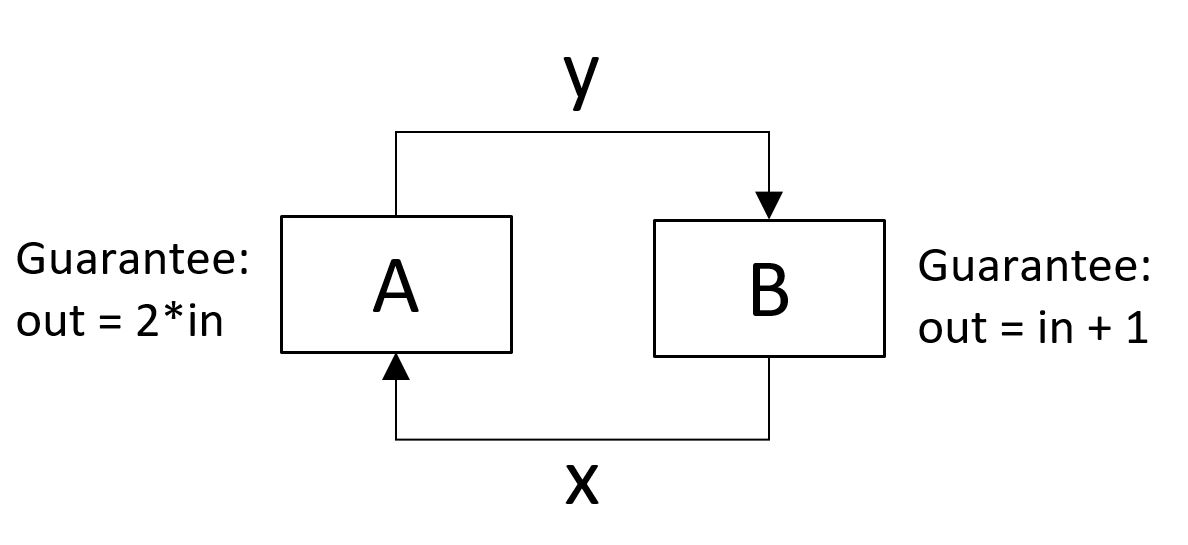
\includegraphics[width=60mm]{simpleFeedback.jpg}
\caption{A Simple Feedback System\label{motivationFig1}}
\end{figure}

First, we will explain the intuition and illustrate the key semantic difference between the synchronous model used in the original AGREE and the proposed model.
Consider an AADL model that consists of two threads $A$ and $B$, shown in Figure \ref{motivationFig1}. Assume all ports are data ports. The behavior of each thread is indicated by its AGREE contract. Thread $A$ output doubles its input. Thread $B$ output increments its input by one. By the synchronous model semantics, the value of signal $x$ and $y$ at instant $n$ is defined by the solution to the two equations $y_n = 2x_n$ and $x_n = y_n+1$, for all $n \in N$. This results in $x = (-1, -1, …)$, $y = (-2, -2, …)$. However, if the two threads execute in a sequential order $(ABAB...)$, and let $x_0, y_0$ denote the initial value of $x$ and $y$, respectively, an intuitive interpretation of the execution semantics is $y_1 = 2x_0, x_1 = y_1+1, y_2 = 2x_1...$. If $x_0 = 0$ and  $y_0 = 0$, this results in $x = (0, 1, 3, 7,…)$ and $y = (0, 0, 2, 6, …)$. The example shows that the behavior of a synchronous model is defined by the solution(s) to systems of mathematical equations (or inequalities) at each instant, while the behavior of the scheduled components is defined through iterations over time. 

\begin{figure}[ht!]
\centering
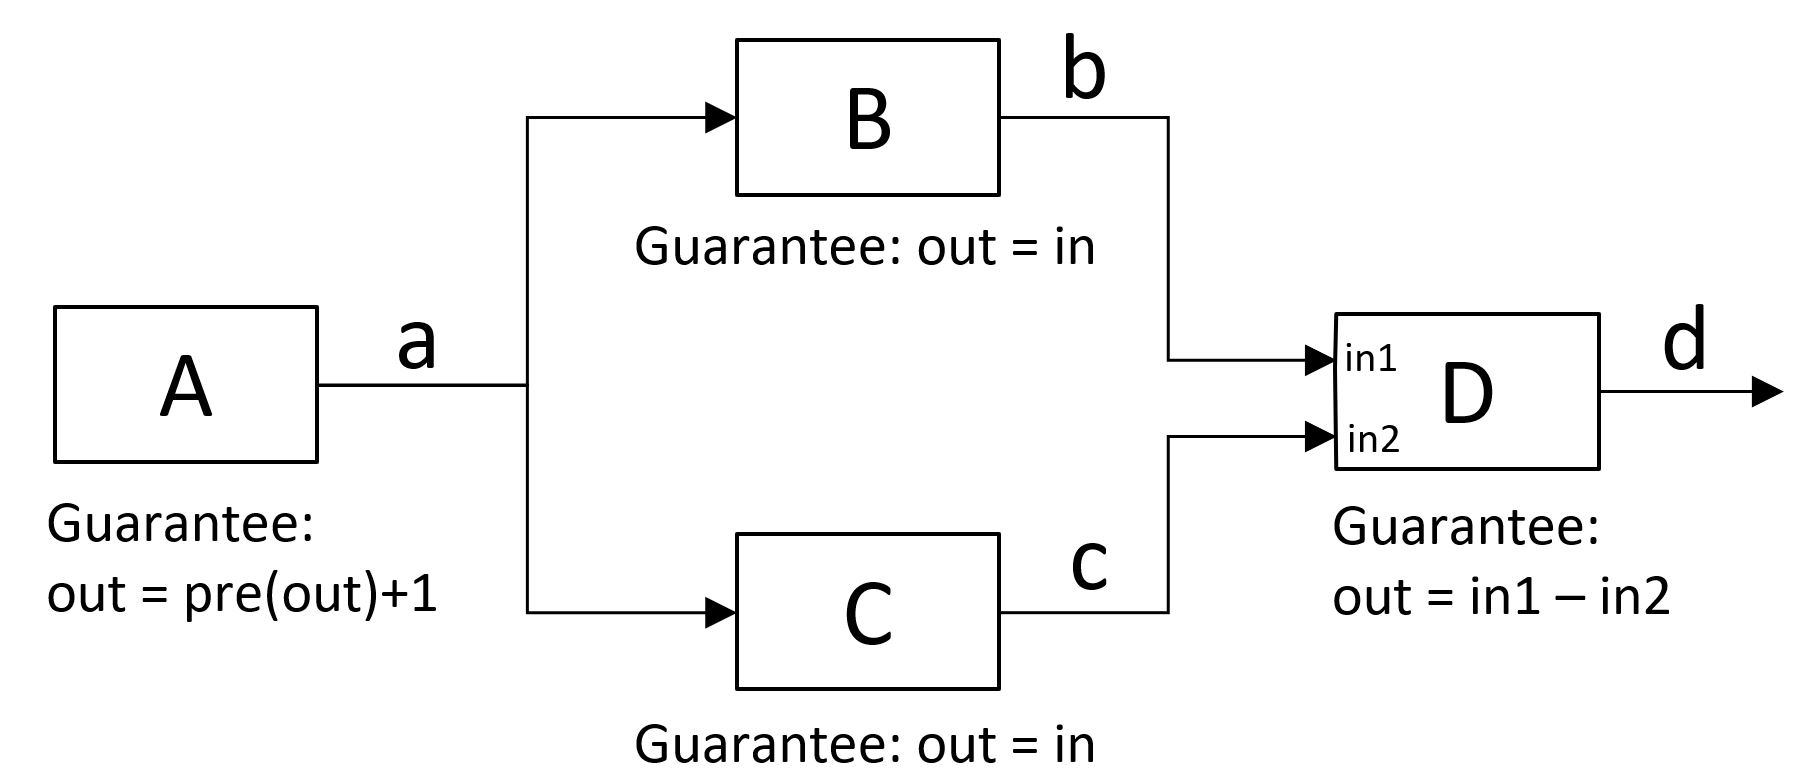
\includegraphics[width=80mm]{downsample.jpg}
\caption{A Simple Downsampling System\label{motivationFig2}}
\end{figure}

Now we will illustrate the motivation of our work.
Consider an AADL model that consists of four threads $A, B, C, D$, shown in Figure \ref{motivationFig2}. Assume all ports are data ports. Thread $A$ outputs the sequence of all natural numbers. Thread B and thread C simply copy its input to the output. Thread D subtracts the second (bottom) input value from the first (top) input value. Given a schedule $(ACABD)^*$, let us say we want to prove that the primary output $d$ is a sequence of ones (ignoring the initial prefix). This can be achieved with the proposed model, since thread $B$ only copies even numbers, and thread $C$ only copies odd numbers. However, it cannot be proved directly with the synchronous model, where $d$ is a sequence of zeroes. To model execution order in a synchronous model, a special construct \emph{delay} is often introduced. However, in the example, thread $B$ and $C$ essentially downsample the data stream from thread $A$. To model this kind of behavior (e.g. downsampling or upsampling), it requires much more complicated modeling mechanism than simple \emph{delays}. 

Note that if the schedule is $(ABCD)^*$, $d$ is a sequence of zeroes (ignoring the initial prefix). This indicates that the execution order could have an impact on the system behavior. As we will show later, our model is not a variant of Kahn Process Network \cite{KPN}, like Lee's Synchronous Dataflow \cite{SDF}, where any execution order results in the same system behavior. Therefore, it makes sense to tie a system-level property to a specific schedule of the components.
%Also note that we could add \emph{assumption: input is an even number} to thread $B$. The assumption has no impact on the system behavior under the proposed MoC. However, under the synchronous AGREE MoC the system has no valid behavior. This is because the assumption is violated under the synchronous semantics. This kind of assumptions are not uncommon. It creates a modelling challenge for using synchronous models. 


 
  

\section{Overview of the Model}
\label{overview}
Now we discuss in details of our semantics interpretation of AGREE contracts with scheduled components.
\begin{figure}[ht!]
\centering
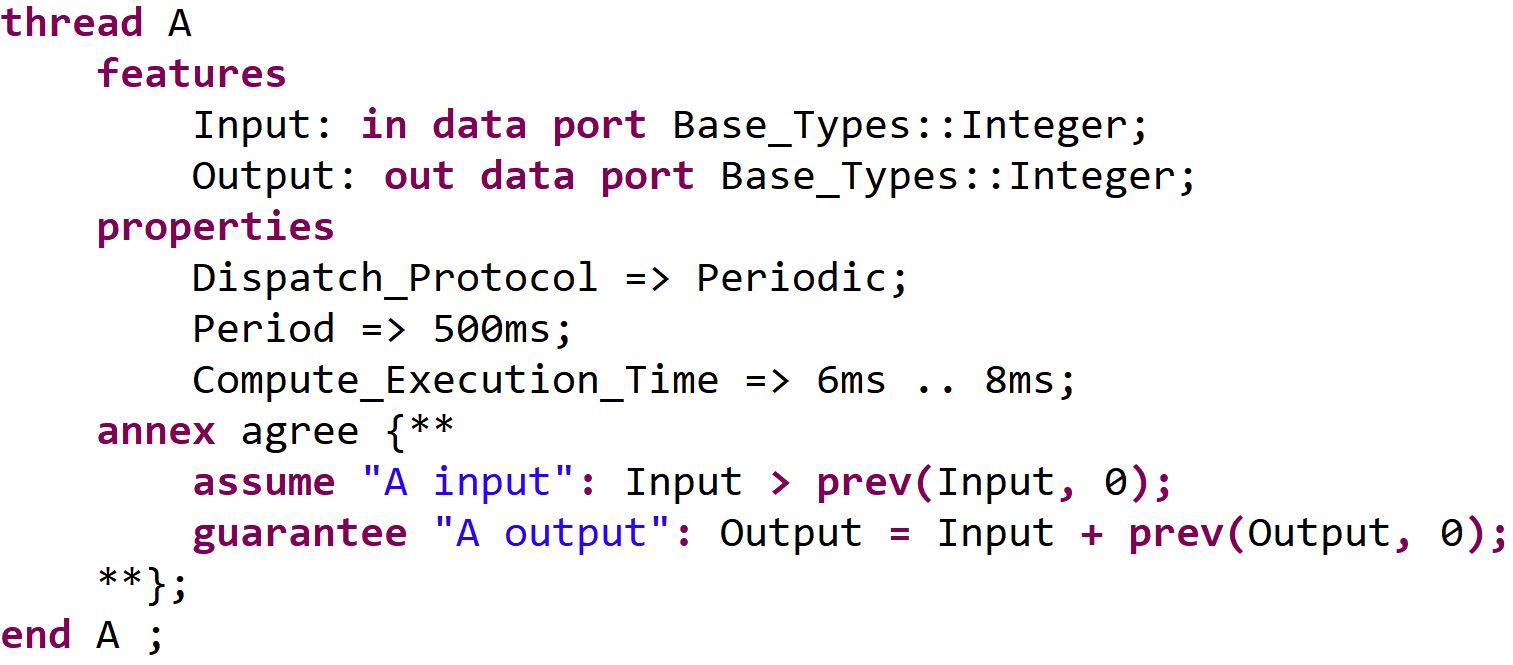
\includegraphics[width=80mm]{pre.jpg}
\caption{A Simple Integrator AADL Model in AGREE\label{integratorFig}}
\end{figure}

First, we use an example to illustrate our rationals. Consider the AADL model of an integrator shown in Figure \ref{integratorFig}. We assume an execution time slot in a schedule is assigned to the thread.  
The first question we have is when the contracts shall hold. In a synchronous model, contracts hold at every instant. However, with scheduled execution, it is reasonable to assume the contract may not hold when the component is not activated. But once it is activated, shall it hold throughout the whole execution or just at certain instants? Second, how shall $Input$ referred in the contract be interpreted? One interpretation is that it refers to the input value at the time when the contract is evaluated, which may vary during the execution. Another interpretation is that it refers to the input value when the component starts its execution. In other words, there is a notion of \emph{sample and hold}. Any input value change during the execution will not impact the current execution. This interpretation is consistent with the notion of \emph{frozen} input described in the AADL V2 standard. Third, how the \emph{prev} operator shall be interpreted? In a synchronous model, it refers to the previous instant. However, with scheduled execution, it seems reasonable to interpret \emph{prev} as previous activation (i.e. the last value when the component was activated). If the contracts hold throughout the activation, a more sensible interpretation is that at the first instant during activation, it refers to the previous activation. Then at each following instant, it refers to the last updated value in the current activation. This interpretation is adopted in the \emph{activation condition} in SCADE \cite{scade} or the \emph{clock} mechanism in SIGNAL \cite{signal}.

AGREE contracts are intended to model requirements \cite{AGREE2}, not implementations. Guarantees model the component requirements, and assumptions models the environmental constraints used to verify the component requirements. Following the AADL \emph{input-compute-output} model, we interpret that the assumptions shall hold at the start of the execution (i.e. \emph{dispatch}) when the inputs are read in. And the guarantees shall be satisfied at the end of the execution (i.e. \emph{complete}) when the outputs are written out. This interpretation has a few implications. 
First, since we adopt the AADL frozen input concept, any reference to $Input$ refers to the input value that was read in at dispatch.
Second, a component's assigned time slot does not necessarily match exactly with its execution time window. If the time slot is greater than its execution time, we interpret the start and end of the time slot as dispatch and complete, respectively. Otherwise, we interpret a preemption has occured.
Third, each contract is examined exactly once in each activation. Thus, we interpret the $prev$ operator as the previous activation. 
Examing guarantees only once means they are not intended to model the transient behavior during an execution. We interpret them as requirements on the steady-state outputs at the end of activation.

%This is different from the real-time behavior models used to formalize AADL semantics, like real-time Maude \cite{maude}, timed automata \cite{behaviorannex}, and timed Petri net \cite{tpn}. They model the component timing behavior throughout the whole execution. 
Note that this does not mean AGREE contracts cannot model timer (or integerator) based requirements. In practice, a timer is usually implemented as a counter, whose limit (constant) is calculated based on the frequency of its execution. The counter is activated periodically and increments by only one during each activation, independent of the execution time. This is consistent with our interpretation.

Thus, we introudce two distinctive events \emph{dispatch} and \emph{complete} for each component to model the start and end of its activation, respectively. 
Similarly, for a system (consists of components), the two events model the start and end of a scheduling cycle. 
The two events shall appear in pairs and alternately. dispatch shall appear before complete. We introduce \emph{well-orderedness} to capture the pattern.

In SCADE and SIGNAL, when a component is not activated, its outputs keep their previous values. We adopt the same notion of output freeze. The outputs are frozen between complete events. 

We inherit the communication mechnanism used in synchronous AGREE. The existence of a connection between two components means their contracts refer to the same variable. 
This essentially simulates an asynchronous communication between components with shared variable. It has one writer and possibly multiple readers. This is consisten with the AADL data port communication semantics.
Since the schedule ensures at most one component is activated at a time, there is no ambiguity on the order of read and write. For a preemptive schedule, we require a component can only be prempted by another component if they do not have connections.

The comminucation may also be viewed as a buffer of size one, which has exactly one writer and one reader. The writer overwrites when overflow occurs. The reader reads the last value if the queue is empty. This means the model only supports restrictive AADL event data port communication.

Following the AADL frozen input concept, we require the inputs values do not change while the component is activated. This implies assumptions could be examined at \emph{complete}, instead of \emph{dispatch}. Thus, we do not necessarily need introducing \emph{dispatch} event. We keep \emph{dispatch} event mainly for usability reasons. The (\emph{dispatch, complete}) pair helps users to understand a counterexample and mentally construct the system trace. This is particularly useful when the schedule is preemptive.

%{\bf Model of Real-Time Schedule.}
In practice, a schedule often orignally comes in form of a sequence of time slots associated wtih components. 
The schedule could come from an AADL real-time scheduling tool like Cheddar \cite{cheddar}, or from a scheduler provided by the RTOS/Microkernel verdor, like seL4 \cite{sel4}. 
To properly model the schedule in AGREE, the component execution time has to be considered. Consider the example shown in Figure \ref{RTschedule}. There are two scheduled components $A$ and $B$. We refer the original schedule as real-time schedule. We refer its model in AGREE as AGREE schedule.
\begin{figure}[ht!]
\centering
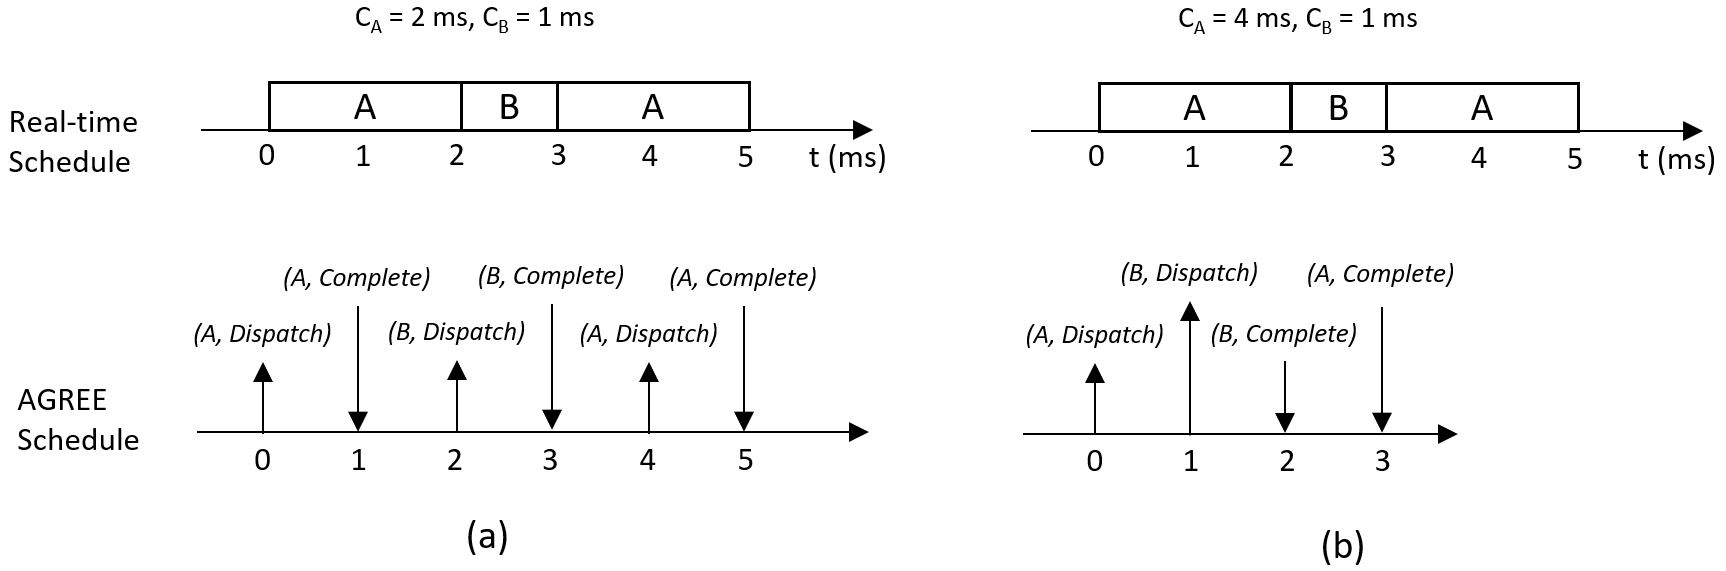
\includegraphics[width=130mm]{RTschedule.jpg}
\caption{A Model of Real-Time Schedule in AGREE\label{RTschedule}}
\end{figure}
Given the same real-time schedule, due to the different execution time $C_A$ of $A$, two different AGREE schedules are created. In Figure \ref{RTschedule}(a), since $C_A$ is equal to the time slots assigned to $A$, the end of the each time slot is modelled as \emph{complete}. In Figure \ref{RTschedule}(b), since the first time slot assigned for $A$ is less than its execution time, the end of the first time slot is interpreted as \emph{preemption}, instead of \emph{complete}.

%The AGREE reasoning framework uses past-time LTL [2], particularly LTL operator $G$ (globally), $H$ (historically), and $Z$ (previous). Given a component with an assume-gurantee pair ($A,P$) and an event pair (\emph{dispatch}, \emph{complete}), the meaning of the contract can be formally represented as a past-time LTL formula $G(H((dispatch \Rightarrow A)) \Rightarrow (complete \Rightarrow P))$. In synchronous AGREE, the two events \emph{collpase} into a single instant at each tick. Thus, we have $G(H(A) \Rightarrow P)$.

%A system consists of components, connections between components, contracts, and a schedule.
%The schedule defines a total order of dispatch and complete events of each component within a scheduling cycle.
%A valid schedule is one where component activations do not overlap.
%Once a component is activated, it runs to complete. There is no preemption.
%A component reads input at dispatch time. %Reading is non-blocking. It reads the most recent input data value or an initial value. 
%And the input is \emph{frozen} during the component activation.
%A component writes output at completion time. %Writing is non-blocking. It overwrites the previous data value. 
%And the output holds its data value between its completions.
%The connections represent an asynchrnous communication channel with a buffer of size one.
%The connections between components are unidirectional. %It represents communication through shared variable with one writer and possible multiple readers. 
%A component satisfies its assumptions at dispatch time. %If the assumption is violated, then the system is consided \emph{inconsistent}.
%A component satisfies its guarantees at completion time. 
%And the output holds its data value between its completions.

%{\bf External Input.} 
System inputs from the environment could arrive at any instant, while the system runs periodically. To avoid missing events, we assume that either there is a buffer mechanism that stores all the input messages on a queue and periodically send it out to the system for processing, or the message arrival is synchronized with the component activation. % We assume the communication can be modelled as a shared variable, and the communication rate is the same as the system execution rate. 



\section{Formal Definitions}
\label{async}

First, we describe the rational behind our semantics interpretation of an AADL model in AGREE with a schedule. Then, we will present the formal definitions and discuss their connection to AADL semantics.

\begin{figure}[ht!]
\centering
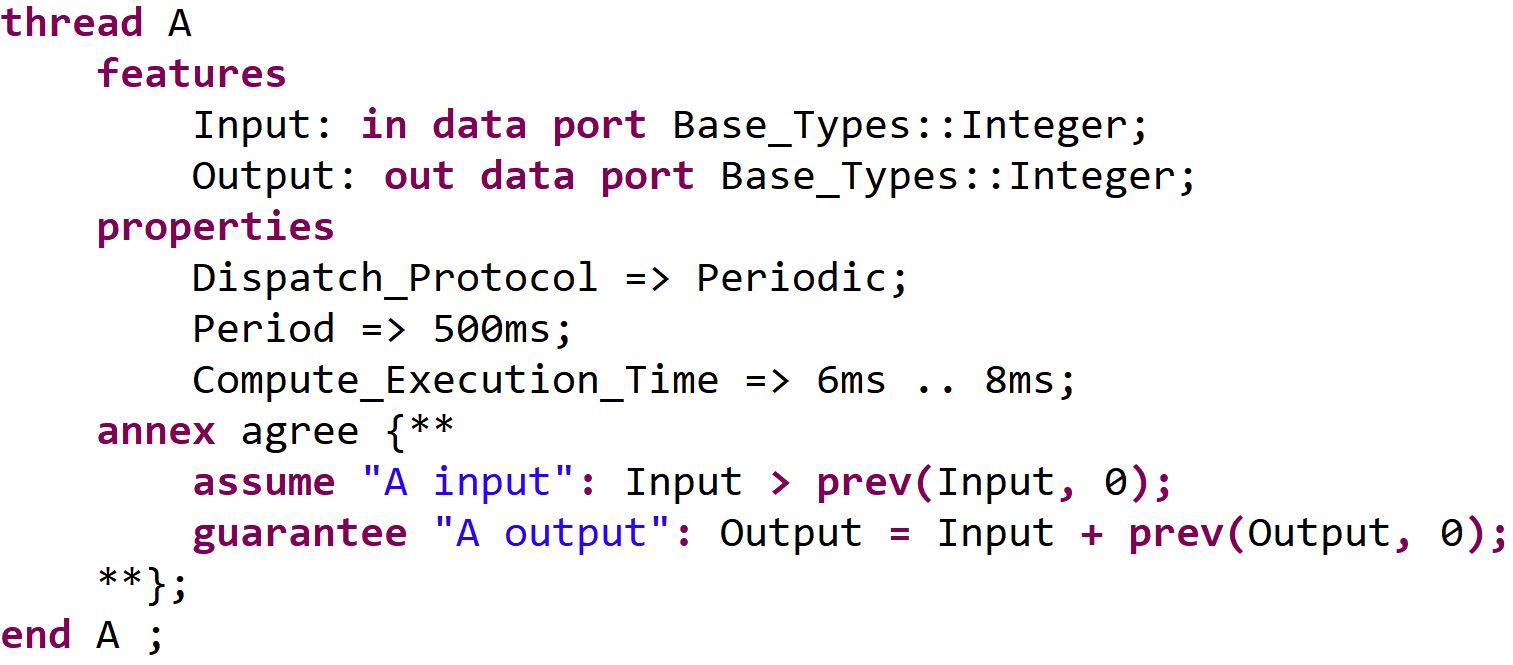
\includegraphics[width=80mm]{pre.jpg}
\caption{A Simple Integrator AADL Model in AGREE\label{integratorFig}}
\end{figure}

We use an example to explain our rationals. Consider an AADL thread with AGREE contracts shown in Figure \ref{integratorFig}. Let us assume a scheduler assigns a time slot to the thread. There are a few questions that need to be clarified before we understand the semantics. 
First, when shall the contracts hold? In a synchronous model, the contract shall hold at every \emph{tick}. However, in a scheduled execution, it is reasonable to assume the contract may not hold when the component is not \emph{active}. But once it is active, shall it hold throughout the whole execution or just at certain instants? 
Second, how shall $Input$ referred in the contract be interpreted? One interpretation is that it refers to the input value at the time when the contract is evaluated, which may vary during the execution. Another interpretation is that it refers to the input value when the component starts its execution. In other words, there is a notion of \emph{sample and hold}. Any input value change after the execution will not impact the current execution. This interpretation is consistent with the notion of \emph{frozen} input in AADL.
Third, how the \emph{pre} operator shall be interpreted? In a synchronous model, it refers to the previous \emph{tick}. However, in a scheduled execution, it seems reasonable to interpret \emph{pre} as the last value when the component was active. The interpretation makes sense if the contract is evaluated only once during the current execution. If the contract is evaluated multiple times, a more sensible interpretation is that at the first evaluation, it refers to the last value from the previous activation. And at all the following evaluations, it refers to the last updated value in the current execution. This interpretation is adopted in the \emph{activation condition} in SCADE \cite{scade} or \emph{clock} in SIGNAL \cite{signal}.

%This interpretation means that the number of evaluation during the execution could have an impact on the final output value. This is illustrated in the integrator example. To match the software behavior, the evaluation interval has to equal the integration step size used in the implementation. 

%In AGREE, the contracts represent requirements and we want to comply with AADL semantics. This has some implictions.  In AADL, inputs are frozen at dispatch time by default. Thus, we interpret the input referred in a contract as the input value at dispatch time. And assumptions on input or its history hold at dispatch time. 
%
%We assume dispatch occurs at the beginning of the time slot and complete occurs at the end. For now, we assume there is no preemption. We will discuss how preemption is handled in Section 4. Note that we use complete to refer to the end of a time slot. It does not necessarily mean the actual execution ends exactly at the end of the time slot. We interpret it as the upperbound of worst case execution time plus some margin. In other words, this is time for sure the computation is complete and the final output data is available. Note that in acutual implementation the output value may vary during the execution. We interpret guarantees as requrirements on the final output. 

In AGREE, the contracts are intended to model requirements \cite{AGREE2}. Assumptions and guarantees correspond to preconditions and postconditions, respectively. Given the AADL \emph{input-compute-output} model, it is reasonable to interpret that the assumptions shall hold at the start of the execution when the inputs are read in. And the guarantees shall be satisfied at the end of the execution when the outputs are written out. In other words, in AGREE, the contracts are not intended to model the timing behavior within an execution. This is different from the real-time behavior models used to model AADL semantics, like real-time Maude \cite{maude}, timed automata \cite{behaviorannex}, and timed Petri net \cite{tpn}. They model the component timing behavior throughout the whole execution. Note that since each contract is evaluated only once in each activation. The $pre$ operator is always interpreted as the last value from the previous activation.

Note that this does not mean AGREE contracts cannot model timer (or integerator)-like requirements. In practice, a timer is usually implemented as a counter, whose limit (constant) is calculated based on the frequency of its execution. The counter is active periodically and increments by only one during each activation, independent of the execution time. 

Thus, in our interpretation, the length of the execution time at each activation, which could vary from one activation to another, is abstracted out. We introudce two distinctive events \emph{dispatch} and \emph{complete} for each component to model the start and end of its each execution, respectively. Similarly, for a system (consists of components), they model the start and end of a scheduling cycle.

%A system consists of components, connections between components, contracts, and a schedule.
%The schedule defines a total order of dispatch and complete events of each component within a scheduling cycle.
%A valid schedule is one where component activations do not overlap.
%Once a component is activated, it runs to complete. There is no preemption.
%A component reads input at dispatch time. %Reading is non-blocking. It reads the most recent input data value or an initial value. 
%And the input is \emph{frozen} during the component activation.
%A component writes output at completion time. %Writing is non-blocking. It overwrites the previous data value. 
%And the output holds its data value between its completions.
%The connections represent an asynchrnous communication channel with a buffer of size one.
%The connections between components are unidirectional. %It represents communication through shared variable with one writer and possible multiple readers. 
%A component satisfies its assumptions at dispatch time. %If the assumption is violated, then the system is consided \emph{inconsistent}.
%A component satisfies its guarantees at completion time. 
%And the output holds its data value between its completions.
{\bf Signal.}
A signal $x$ is a function of the form $x: N \mapsto T_x$, where $N$ is the set of natural numbers including zero, and $T_x$ is the data type of $x(i)$ for all $i \in N$.
$x(i)$, an assignment of a vlaue in $T_x$ to $x$, is called a \emph{valuation} of signal $x$. A signal represents a possibly infinite sequence of values.
%The data type can be either a primitive data type (e.g. real, bool, int, and enumeration types) or a composite data type (e.g. record types). 
%Assume the data type of signal $x$ and $y$ is $T_x$ and $T_y$, respectively, $x = y$ means that $T_x=T_y$ and $x_i = y_i$ for all $i \in N$. 

{\bf Port.}
Input ports $X = \{x_1, x_2, ..., x_M\}$, where $x_i$ is the \emph{i}-th input port, and $M\in N$ is the total number of input ports. Each port $x \in X$ is associated with a signal. We may use input port or input signal interchangablely. To simplify the notation, we use the port ID $x$ to denote the associated \emph{signal}. Outputs are defined similarly: $Y = \{y_1, y_2, ..., y_K\}$, where $K\in N$ is the total number of output ports.  
A \emph{valuation} of input ports is the valuation of all input signals. That is, $I(n) = \{x_1(n), x_2(n), ... x_N(n)\}$, where $n \in N$. Similarly, a \emph{valuation} of output ports $O(n) = \{y_1(n), y_2(n), ... y_N(n)\}$, where $n \in N$. 

We model the AADL ports as signals. In particular, an event port is modelled as a Boolean signal. The value \emph{1} or \emph{0} indicates the event is \emph{present} or \emph{absent} at the port, respectively. 
An event data port is modelled as a pair of data signal and event signal.  %An event data port is modelled as a pair of data signal $p$ and event signal $event(p)$.  

{\bf Component.}
A component $c$ is a nine-tuple $(S, s_0, I, O, \delta, A, P, dispatch, complete)$, where: 
\begin{itemize}
    	\item $S$ is a finite non-empty set of states;
    	\item $s_0 \in S$ is the initial state;
    	\item $I$ is a set of input signals valuations;
    	\item $O$ is a set of output signals valuations;
    	\item $\delta$ is the state transfer function of the form $\delta: I \times S \mapsto S$;
    	\item $A$ is a set of \emph{assumptions}, for all $a \in A$, $a$ is a Boolan function $I \times S \mapsto B$;
    	\item $P$ is a set of \emph{gurarantees}, for all $p \in P$, $p$ is a Boolan function $I \times O \times S \mapsto B$;
    	\item $dispatch$ is a Boolean signal;
	\item $complete$ is a Boolean signal.
%	\item $clock$ is a Boolean signal $clock(n) \Rightarrow \lnot clock(n+1) \land  \lnot clock(n-1), \forall i \in N$ .
\end{itemize}

Let $s$ be a \emph{valuation} of $S$. That is, $s: N \mapsto S$. We have $ s(n+1) = \delta (s(n), I(n))$.

Note that the guarantees represent a general relation, not a function. This allows users to models the non-derterminism introduced by design decision or implementation choice.
  
%The ports of a thread are divided into two finite disctinct sets: input ports ($I$) and output ports ($O$). Correspondingly, the associated signals are divided int to input signals and output signals. We model the \emph{state} of a thread with a finite set $S$ of signals. %The next state function is $T: S x I \mapsto S'$. The output function is $T: S x I \mapsto S$. Then, a thread is %A thread is modelled as a collection of input signals and output signals. A thread could be aossciated with /emph{local} states, which are not accessible outside the scope of the thread. They are modelled as signals, noted as set S . 

%{\bf component execution.}

%A component is associated with two Boolean signals (events) \emph{dispatch} ($d$) and \emph{complete} ($c$). A component is \emph{dispatched} at time $i$, if and only if $d(i) = true$. A component is \emph{complete} at time $i$, if and only if $c(i) = true$. %A component can be in either \emph{active} or \emph{sleep} mode. 
%At \emph{dispatch} a component evaluates the inputs. At \emph{complete}, it updates its output and transitions to its \emph{next state}. After \emph{complete}, it holds its state and output till next \emph{complete}. That is,

%A \emph{valuation} of an assumption $a$ is defined as $a(n) =  a(I(n), s(n))$.
%A \emph{valuation} of a gurarantee $p$ is defined as $p(n) =  p(I(n), O(n), s(n))$.

At \emph{dispatch}, the \emph{assumptions} $A$ should hold. That is,

\begin{equation} 
\label{eqn:assumption}
dispatch(n) \Rightarrow a(I(n), s(n)), \forall n\in N, \forall a \in A
\end{equation}

At \emph{complete}, the \emph{gurarantees} $P$ should hold. That is,

\begin{equation} 
\label{eqn:guarantee}
complete(n) \Rightarrow p(I(n), O(n), s(n)), \forall n\in N, \forall p \in P
\end{equation}

A compoent holds its state and output between \emph{complete}. That is,

\begin{equation} 
\label{eqn:outputhold}
\lnot complete(n) \Rightarrow y(n) = y(n-1), \forall n \in N, \forall y \in Y
\end{equation}

\begin{equation} 
\label{eqn:statehold}
\lnot complete(n) \Rightarrow s(n) = s(n-1), \forall n \in N, \forall s \in S
\end{equation}

%The \emph{dispatch} and \emph{complete} models, respectively, the start and end of the time slot that a component to run. 
%When its \emph{dispatch} event $d$ is present, a thread samples the input values and starts execution. This is the time when the associated AGREE \emph{assumptions} $A$ should hold. That is,
%$$event(d)_i \Rightarrow a_i, \forall i\in N, \forall a \in A $$

{\bf Trace.}
A trace $\sigma$ of a component $c(S, s_0, I, O, \delta, A, P, dispatch, complete)$ is a function of the form $\sigma: N \mapsto \Sigma$, where
$\sigma(n) = ((I(n), O(n), s(n), dispatch(n), complete(n))$, for all $n\in N$, that satifies Equation \ref{eqn:assumption}, \ref{eqn:guarantee}, \ref{eqn:outputhold}, \ref{eqn:statehold}. %We denote the set of all traces of a component as $\Sigma$.
A trace is a possibly infinite sequence of component valuations that satify the contract constraints and the output and state hold rules. 

{\bf Connection.}
Suppose component $c$ has output ports $Y$ and component $c', c' \neq c$ has input ports $X$. A connection $e$ is a Boolean function: $Y \times X' \mapsto B$. In AGREE, we have
\begin{equation} 
\label{eqn:connection}
e(y, x') \Rightarrow y = x', \forall y \in Y, \forall x \in X'
\end{equation} 

A \emph{connection} from an output port of one component to an input port of another component implies the corresponding signals are equal. For an AADL event data prot, this means the data signals and event signals are equal, respectively. 

%The trace of the simple downsampling system is shown in Table \ref{tab:table1}.
%\begin{table}[h!]
%\begin{center}
%\caption{A Simple Downsampling System Trace}
%\label{tab:table2}
%\begin{tabular}{ |c|c|c|c|c|c|c|c|c|c|c|c| } 
%\hline
%k & 0 & 1 & 2 & 3 & 4 & 5 & 6 & 7 & 8 & 9 & 10 \\
%\hline
%a(k) & 0 & 1 & 2 & 3 & 4 & 5 & 6 & 7 & 8 & 9 & 10 \\
%\hline
%b(k) & 0 & 1 & 2 & 3 & 4 & 5 & 6 & 7 & 8 & 9 & 10 \\
%\hline
%c(k) & 0 & 1 & 2 & 3 & 4 & 5 & 6 & 7 & 8 & 9 & 10 \\
%\hline
%d(k) & 0 & 0 & 0 & 0 & 0 & 0 & 0 & 0 & 0 & 0 & 0 \\
%\hline
%\end{tabular}
%\end{center}
%\end{table}}

Figure \ref{wpmAGREE} shows an exmaple of direct modelling the component semantics in the AADL AGREE annex. This is mostly done by augumenting the contracts defined in synchronous AGREE, and adding additional contracts to enforce the output hold rule.

\begin{figure}[ht!]
\centering
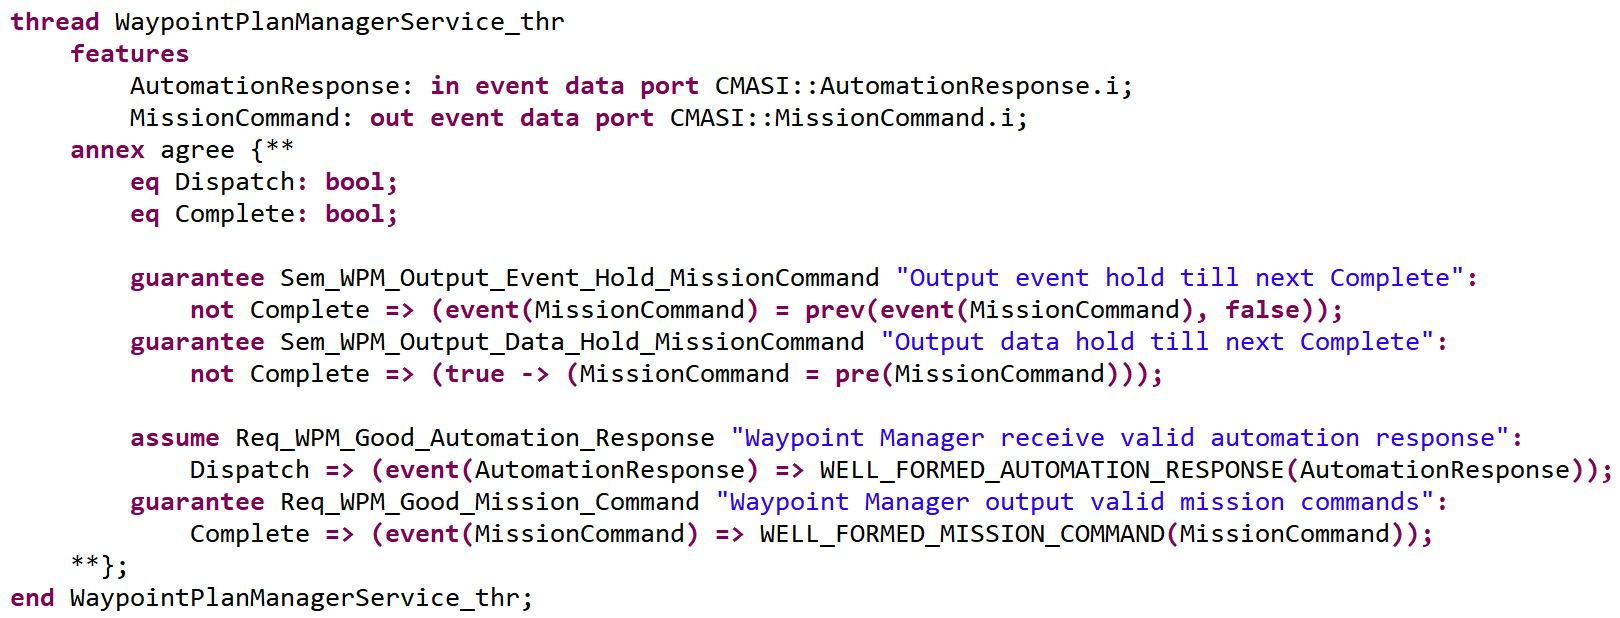
\includegraphics[width=130mm]{wpmAGREE.jpg}
\caption{An AGREE Model Example\label{wpmAGREE}}
\end{figure}

{\bf Schedule.}
Let $C$ be a finite set of components, a schedule $\phi$ of $C$ with \emph{length} $T\in N$ is a partial function $T \mapsto C\times \{Dispatch, Complete\}$ satisfying:
\begin{itemize}
	\item there exists $i\in T$, $c\in C$ such that $\phi(i) = (c, Dispatch)$ if and only if there exists $j\in T$, such that $j > i, \phi(j) =  (c, Complete)$.
	\item if there exists $i, j\in T$, $c\in C$ such that $i \neq j, \phi(i) = (c, Dispatch), \phi(j) = (c, Dispatch)$, then there exists $k\in T$, such that $j >k> i, \phi(j) =  (c, Complete)$.
\end{itemize}
The first condition requires that in a schedule \emph{Dispatch} and \emph{Complete} of a component must appear in pairs, and in each pair \emph{Dispatch} appears ``before'' \emph{Complete}. The second condition states that \emph{Dispatch} and \emph{Complete} of a component must appear alternately in a schedule. 

Then given a schedule $\phi$ of components $C$, the \emph{dispatch} and \emph{complete} signal of a component $c \in C$ can be defined as:
  
\begin{equation}
\label{eqn:dispatch}
    dispatch(i+kT) =
    \begin{cases}
      1, & \text{if}\ \phi(i) = (c, Dispatch) \\
      0, & \text{otherwise}
    \end{cases}
\end{equation}

\begin{equation}
\label{eqn:complete}
    complete(i+kT) =
    \begin{cases}
      1, & \text{if}\ \phi(i) = (c, Complete) \\
      0, & \text{otherwise}
    \end{cases}
\end{equation}

where $i,k\in N$.
A schedule is \emph{fair} if $\phi$ is \emph{surjective}. This means that every component is executed at least once.
A schedule is \emph{minimal} if $\phi$ is a \emph{total} function. This means that at each ``tick'' there is a \emph{dispatch} or \emph{complete} event. Note in a synchronous model, a tick represents a global clock that triggers all components to update. While in the proposed model, ticks are used to represent the total order of events. 

With the output hold, the \emph{connection} definition, and the scheudling semantics, we essentially define an asynchronous communication with shared variable. It has one writer and possibly multiple readers. Since the schedule ensures at most one component is active at a time, there is no ambiguity on the order of read and write. The comminucation may be viewed as a queue of size one, which has exactly one writer and one reader. The writer overwrites when overflow occurs. The reader reads the last value if the queue is empty.

{\bf System.}
A \emph{system} is a triple $(C, E, \phi)$, where:
\begin{itemize}
    	\item $C$ is a finite non-empty set of components;
    	\item $E$ is a set of connections;
    	\item $\phi$ is a schedule.
\end{itemize}
A \emph{trace} of a system is a trace of it components that satisfies the connection Equation \ref{eqn:connection} for all $e in E$, and the schedule Equation \ref{eqn:dispatch} and Equation \ref{eqn:complete}.
An \emph{observal trace} of a system is a trace of the system that only has the input and output trajectory.
A trace of the simple downsampling system is partially shown in Table \ref{tab:table1}.

\begin{table}[h!]
\begin{center}
\caption{A Simple Downsampling System Trace}
\label{tab:table1}
\begin{tabular}{ |c|c|c|c|c|c|c|c|c|c|c|c|c|c|c|c|c|c|c|c|c|} 
\hline
            k & 0 & 1 & 2 & 3 & 4 & 5 & 6 & 7 & 8 & 9 & 10  & 11 & 12 & 13 & 14 & 15 & 16 & 17 & 18 & 19 \\
\hline
dispatchA  & 1 & 0 & 0 & 0 & 1 & 0 & 0 & 0 & 0 & 0 & 1 & 0 & 0 & 0 & 1 & 0 & 0 & 0 & 0 & 0  \\ 
\hline
completeA & 0 & 1 & 0 & 0 & 0 & 1 & 0 & 0 & 0 & 0 & 0 & 1 & 0 & 0 & 0 & 1 & 0 & 0 & 0 & 0  \\ 
\hline
dispatchB & 0 & 0 & 0 & 0 & 0 & 0 & 1 & 0 & 0 & 0 & 0 & 0 & 0 & 0 & 0 & 0 & 1 & 0 & 0 & 0  \\ 
\hline
completeB & 0 & 0 & 0 &0 & 0 & 0 & 0 & 1 & 0 & 0 & 0 & 0 & 0 & 0 & 0 & 0 & 0 & 1 & 0 & 0 \\ 
\hline
dispatchC & 0 & 0 & 1 & 0 & 0 & 0 & 0 & 0 & 0 & 0 & 0 & 0 & 1 & 0 & 0 & 0 & 0 & 0 & 0 & 0  \\ 
\hline
completeC & 0 & 0 & 0 & 1  & 0 & 0 & 0 & 0 & 0 & 0 & 0 & 0 & 0 & 1 & 0 & 0 & 0 & 0 & 0 & 0 \\ 
\hline
dispatchD & 0 & 0 & 0 & 0 & 0 & 0 & 0 & 0 & 1 & 0 & 0 & 0 & 0 & 0 & 0 & 0 & 0 & 0 & 1 & 0 \\ 
\hline
completeD & 0 & 0 & 0 & 0  & 0 & 0 & 0 & 0 & 0 & 1 & 0 & 0 & 0 & 0 & 0 & 0 & 0 & 0 & 0 & 1 \\ 
\hline
a(k) & 0 & 1 & 1 & 1 & 1 & 2 & 2 & 2 & 2 & 2 & 2 & 3 & 3 & 3 & 3 & 4 & 4 & 4 & 4 & 4 \\
\hline
b(k) & 0 & 0 & 0 & 0 & 0 & 0 & 0 & 2 & 2 & 2 & 2 & 2 & 2 & 2 & 2 & 2 & 2 & 4 & 4 & 4 \\
\hline
c(k) & 0 & 0 & 0 & 1 & 1 & 1 & 1 & 1 & 1 & 1 & 1 & 1 & 1 & 3 & 3 & 3 & 3 & 3 & 3 & 3 \\
\hline
d(k) & 0 & 0 & 0 & 0 & 0 & 0 & 0 & 0 & 1 & 1 & 1 & 1 & 1 & 1 & 1 & 1 & 1 & 1 & 1 & 1 \\
\hline
\end{tabular}
\end{center}
\end{table}

{\bf Assume-Guarantee Reasoning.}
Given a system and a set of system \emph{assumptions} $A_s$ and a \emph{guarantee} $p_s$, a \emph{trace} of the contract is a sequence of inputs and outputs valuations that satisfies:

\begin{equation} 
\label{eqn:sys_assumption}
dispatch_s(n) \Rightarrow a_s(n), \forall n\in N, \forall a_s \in A_s
\end{equation}

\begin{equation} 
\label{eqn:sys_assumption}
complete_s(n) \Rightarrow p_s(n), \forall n\in N
\end{equation}

where:
\begin{equation}
\label{eqn:sys_dispatch}
    dispatch_s(n) =
    \begin{cases}
      1, & \text{if}\ n = kT, k=0,1,... \\
      0, & \text{otherwise}
    \end{cases}
\end{equation}

\begin{equation}
\label{eqn:sys_complete}
    complete_s(n) =
    \begin{cases}
      1, & \text{if}\ n = kT-1, k=1,2,... \\
      0, & \text{otherwise}
    \end{cases}
\end{equation}

Verifying a system satisfies its contract $(A_s, p_s)$ is to check whether the set of traces of the contract is a subset of the oberservable traces of the system. TODO

{\bf Hierarchical Composition.}
The proposed semantics supports hierarchical composition. This is possible if the structural proximity of the models is coincidental with the temporal proximity of their time slots in a schedule. We illustrate this using the example shown in Figure \ref{pic:hierarchy}. A system $G$ consists of components $A$ and $B$. Suppose given the lower-level schedule $(ABA)$, we prove the contracts of $G$. Then, at the structural higher-level, $G$ could be viewed as a component. And since component $A$ and $B$ are also scheduled to execute one after another, $G$'s time slot is the concatenation of the time slots of its components. Thus its \emph{dispatch} and \emph{complete} events is the start and end of the combined time slot, respectively.

\begin{figure}[ht!]
\centering
\includegraphics[width=100mm]{Hierarchy.jpg}
\caption{An Example of Hierarchical Composition in AGREE\label{pic:hierarchy}}
\end{figure}

Note that if all the inputs of a component are connected to the outputs of other components, the inputs value will not change while the component is active. This is because the other components hold their outputs while inactive. It implies assumptions could be checked at \emph{complete}, instead of \emph{dispatch}. Thus, we do not necessarily need \emph{dispatch} event for verification purposes. Actually, in the backend implementation, assumptions at checked at \emph{complete}. We keep \emph{dispatch} event mainly for usability reasons. The (\emph{dispatch, complete}) pair helps users to understand a counterexample and mentally construct the system trace. This is particularly useful when the schedule is preemptive .

{\bf Model of Real-Time Schedule.}
In practice, a schedule often comes in form of real-time schedule, a sequence of time slots associated wtih components. The real-time schedule could come from an AADL scheduling tool like Cheddar \cite{Cheddar}, or from a scheduler provided by the RTOS/Microkernel verdor, like seL4\cite{seL4}. To properly model the schedule in AGREE, the component execution time has to be considered. One example is shown in Figure \ref{RTschedule}, where there are two components $A$ and $B$. 
\begin{figure}[ht!]
\centering
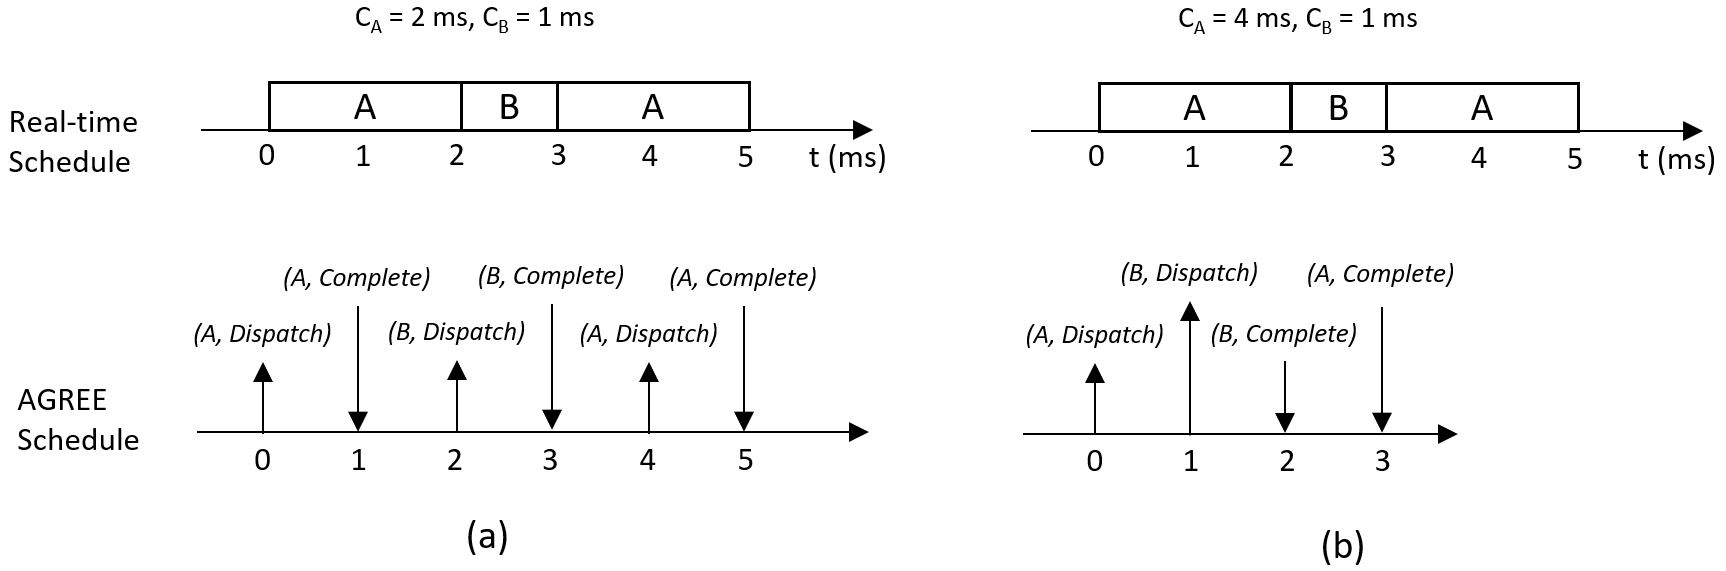
\includegraphics[width=130mm]{RTschedule.jpg}
\caption{A Model of Real-Time Schedule in AGREE\label{RTschedule}}
\end{figure}
Given the same real-time schedule, due to the different execution time $C_A$ of $A$, different AGREE schedules are created. In Figure\ref{RTschedule}(b), since the first time slot assigned for $A$ is less than its execution time, the end of the first time slot is interpreted as \emph{preemption}, instead of \emph{complete}.

We introduce a circular counter to model a schedule in AGREE. The maximum count models the period of the schedule. An AGREE model of the schedule $(ABACD)^*$ used in the example is shown in Figure \ref{schedule}.
\begin{figure}[ht!]
\centering
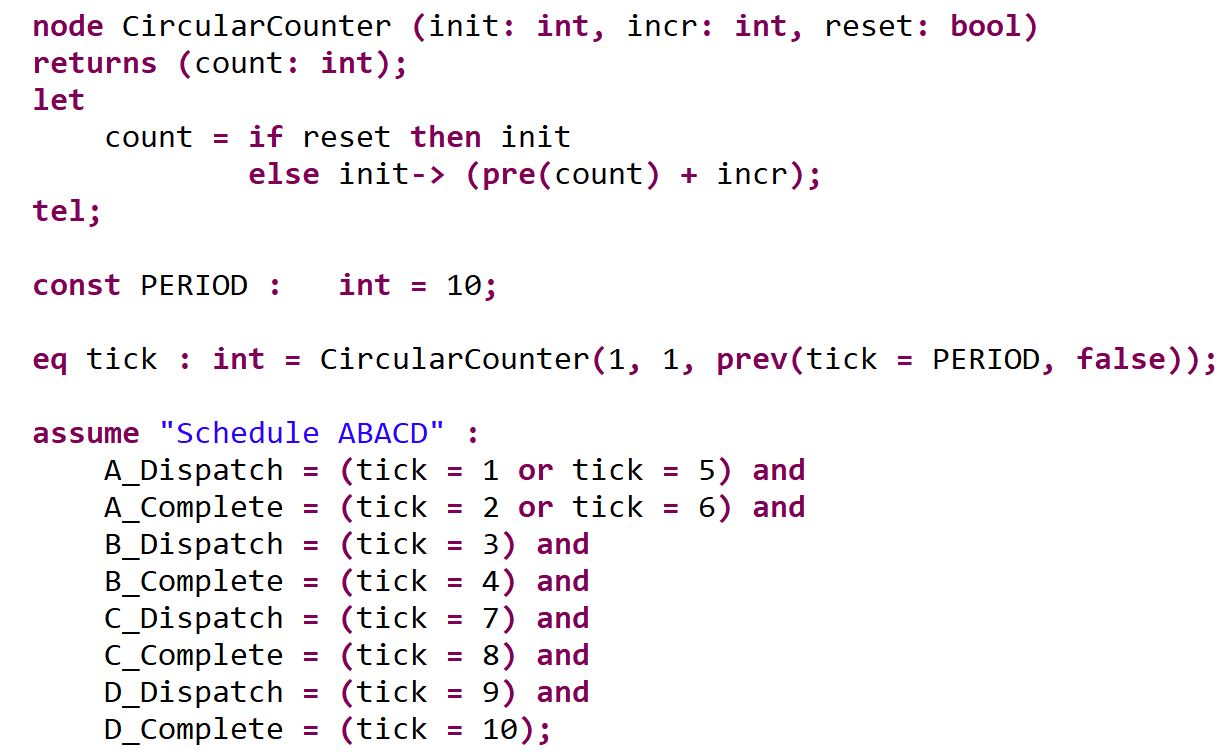
\includegraphics[width=100mm]{schedule.jpg}
\caption{A Model of Schedule in AGREE\label{schedule}}
\end{figure}


%An AGREE model of the schedule $(ABACD)^*$ used in the example is shown in code~\ref{schedule_model}

%\begin{lstlisting}[language=c,frame=single,caption=An AGREE model of a schedule,label=schedule_model]
%node CircularCounter (init: int, incr: int, reset: bool)	
%returns (count: int);
%let
%	count = if reset then init
%		else init-> (pre(count) + incr);
%tel;
%				
%eq tick : int = CircularCounter(1,1,prev(tick=10,false));
%
%assume "Schedule ABACD" :
%	A_dispatch = (tick = 1 or tick = 5) and
%	A_complete = (tick = 2 or tick = 6) and					
%	B_dispatch = (tick = 3) and	
%	B_complete = (tick = 4) and
%	C_dispatch = (tick = 7) and
%	C_complete = (tick = 8) and	
%	D_dispatch = (tick = 9) and
%	D_complete = (tick = 10);			
%\end{lstlisting}	

%The model of a schedule can be simplified to potentially improve the formal verification performance. The thread execution time can be modelled as just one tick. The idle time or communication delay can be abstracted out. For the same example above, a simplified schedule could be  $\phi' = \{d(A)=(1,0,0)^*, c(A) = (0,1,0)^*, d(B) = (0,1,0)^*, c(B) = (0,0,1)^*\}$. The intuition is that as long as the execution order is preserved, the verfication problem of such a model is equavilent to that of a model directly mapping each base time unit to a tick. 
%	
%\begin{theorem}
%Given an AADL model with two \emph{equavilent} schedules $\phi$ and $\phi'$, a property of the model holds under schedule $\phi$ if and only if it hold under schedule $\phi'$.
%\end{theorem}
%
%{\bf Proof sketch.} 
%It is possible to show that any counter-example found in the proof of the system property of model with schedule $\phi$ can be mapped to a counter-example of the proof of the same system property of the same model with schedule $\phi'$,  and vice versa.  

{\bf External Input.} 
System inputs from the environment could arrive at any instant, while the system runs periodically. To avoid missing events, we assume that there is a buffer mechanism that stores all the input messages on a queue and periodically send it out to the system for processing. We assume the communication can be modelled as a shared variable, and the communication rate is the same as the system execution rate. 

%\documentclass{article}
%\usepackage{multirow}
%\begin{document}
%\begin{center}
%\begin{tabular}{ |c|c|c|c|c|c|c|c|c|c|c|c| } 
%\hline
%k & 0 & 1 & 2 & 3 & 4 & 5 & 6 & 7 & 8 & 9 & 10 \\
%\hline
%& Active & - & A & B & A & C & D & A & B & A & C & D \\ 
%\hline
%\end{tabular}
%\end{center}
%\end{document}

%As suggested by previous examples, the schedule or execution order has an impact on the system behavior. This differs from other dataflow models, such as Synchronous Dataflow \cite{sdf}, or other variants of Kahn Process Networks \cite{kpn}. It is known 

%{\bf model of execution delay.}
%The thread exeution delay is not directly modelled. Instead, the time slot allocated to a thread in a schedule is modelled by the \emph{distance} between the thread \emph{dispatch} and \emph{complete}. If we assume there is no pre-emption, this modells  the worst case execution time or deadline.

%{\bf model of communication delay.}
%The communication delay is abstracted out. However, in a schedule there is often a time window between the complete event of the one thread and the dispatch event of the next thread. This time window models the %worst case communication delay.

%{\bf AGREE contracts.}

%Our approach to modelling the AADL asynchronous MoC in AGREE is to keep the existing AADL model structure intact and add new AGREE contracts and augument existing contracts. The added contracts model the asynchronous communication between AADL ports. The modification of the exisiting contracts reflcts the interpretation of the contracts under the asychronous AGREE MoC. 

%\begin{figure}[ht!]
%\centering
%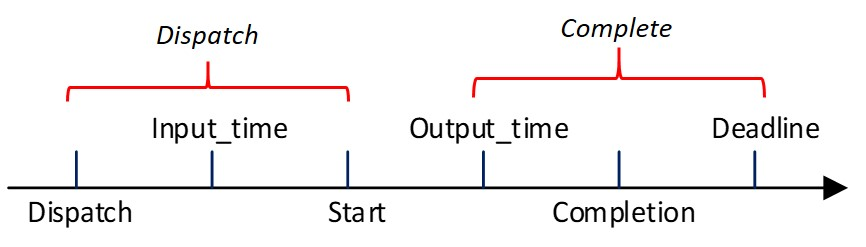
\includegraphics[width=80mm]{aadl_events.jpg}
%\caption{An AADL Model with AGREE Contracts\label{motivation}}
%\end{figure}

%In asynchronous AGREE, the \emph{Execution\_Time} property is modelled by the time interval between the \emph{Dispatch} event and the \emph{Complete} event.
%The assumptions hold at the \emph{Dispatch} event \[Dispatch => Assumption\] , and the guarantees hold at the \emph{Complete} event, i.e. \[Complete => Guarantee\] 
%
%% Assumptions
%We make the following assumptions. The \emph{Input\_Time} property value is unspecified, thus default to dispatch time. The \emph{Output\_Time} property value is unspecified, thus default to the execution completion time. The \emph{Queue\_Size} property value is unspecified, thus default to size one. The \emph{Execution\_Time} property represent a single value, not a real range. The \emph{Dispatch\_Protocol} property value is periodic. The \emph{Timing} property value of each connection is unspecified, thus default to immediate connection. There is no simultaneous read and write access to a queue or buffer (data port). If an event data queue or a data port buffer is empty, the most recent data is used. The \emph{Dequeue} occurs at every dispatch. There is no preemption. There is no propagation delay.
%
%% Modelling
%For an output event data port of a thread, the event and data holds till the thread's next \emph{Complete} event. This is represented by the following AGREE contracts.
%
%\begin{math} 
%not Complete => (event(Port) = prev(event(Port), false))
%\end{math} 
%
%\begin{math}
%not Complete => (true -> (Port = pre(Port)))
%\end{math}  
%
%% Rational
%The output event hold models the latching behavior of an event queue (size one). At the end of execution of a thread, an output event may or may not be raised. However, the AGREE contracts representing the functional requirements only ensures an event is raised only at that exact time instant (i.e. \emph{Complete}). The event is latched so that the target thread, once dispatched, samples the correct result. The consideration for the output data hold is similar.
% 
%% Schedule
%In asynchronous AGREE, a schedule defines the sequential execution order of threads. It is specified by the user. It often come from the actual software execution schedule on the target platform (e.g. seL4 domain schedule). Currently AADL does not define a standard format to specify a schedule. We used AGREE \emph{assumption} on each thread's \emph{Dispatch} and \emph{Complete} event to represent a schedule. For example, \emph{assume "schedule" :			ThreadA\_Dispatch = (Frame = 60) and ThreadA\_Complete = (Frame = 70) and ...}



%\section{Verification Conditions for Async AGREE}
\section{Assume-Guarantee Reasoning}

\newcommand{\globally}{\ensuremath{\mathbf{G}}}
\newcommand{\historically}{\ensuremath{\mathbf{H}}}
\newcommand{\assumes}{\ensuremath{A}}
\newcommand{\guarantees}{\ensuremath{P}}
\newcommand{\dispatch}{\ensuremath{\mathit{dispatch}}}
\newcommand{\complete}{\ensuremath{\mathit{complete}}}
\newcommand{\same}[1]{\ensuremath{\mathit{same}(#1)}}
\newcommand{\inputs}{\ensuremath{I}}
\newcommand{\outputs}{\ensuremath{O}}
\newcommand{\system}{\ensuremath{S}}
\newcommand{\components}{\ensuremath{C}}
\newcommand{\schedule}{\ensuremath{\phi}}
\newcommand{\valid}{\ensuremath{\mathit{valid}}}
\newcommand{\dpred}{\ensuremath{\delta^\phi}}
\newcommand{\dispred}{\ensuremath{\mathbb{D}^\phi}}
\newcommand{\compred}{\ensuremath{\mathbb{C}^\phi}}

Scheduled components lend themselves to hierarchical assume-guarantee reasoning in a manner similar to that in~\cite{AGREE2}.
The verification conditions to prove a system of unscheduled components correct are formalized in \emph{past-time linear temporal logic} (PLTL). 
The two PLTL operators necessary for the verification conditions are $\globally$ (globally) and $\historically$ (historically).
These are defined over a trace of the system, $\pi$, and a moment of evaluation in the trace, $i$, as follows:
\begin{eqnarray*}
 (\pi, i) \models \globally(f) & \iff & \forall j \ge i, (\pi, j) \models f \\
(\pi, i) \models \historically(f) & \iff & \forall 0 \le j \le i, (\pi, j) \models f
\end{eqnarray*}
Globally is invariant from the current moment into the future and historically is invariant from the beginning to the current moment.

We define $\mathbb{I}_c$ to be the set of components providing input to some component $c$ in the system, and we define $\mathbb{O}$ to be the set of components that provide the output for the system. An unscheduled system, $\system = (\inputs, \outputs, \assumes, \guarantees)$, is correct if and only if for all $\pi$ and for all $i \ge 0$ the following holds:
\[
\begin{array}{lll}
        & \forall c \in \components &  
            \globally(\historically(\assumes \wedge 
            \bigwedge_{c^\prime \in \mathbb{I}_c} P_{c^\prime}) 
            \implies \assumes_c) \\
 \wedge &   & 
            \globally(\historically(\assumes \wedge 
            \bigwedge_{c^\prime \in \mathbb{O}} \guarantees_{c^\prime}) 
            \implies \guarantees)
\end{array}
\]
The first condition checks the input assumptions on each component under the system assumptions and upstream component guarantees. The second checks the output guarantees of the system under the system assumptions and component guarantees providing the output.  If both conditions hold, then the system is said to be \emph{correct}, meaning that $\globally(\historically(\assumes) \implies \guarantees)$ holds.

The verification conditions are extended to scheduled components by adding a notion of \textit{dispatch} and \textit{complete} to the verification conditions.
We define a predicate $\same{X}$ that is true in the first moment, and after that, true is any moment if and only if the signals in the set $X$ are unchanged from the previous moment.
We also define the predicate $\dpred_c$ to be true if the current moment is in a dispatch interval for the component $c$ according the schedule.

The assumptions in a scheduled component hold at dispatch, and the guarantees of the same component hold at complete.
A component also assumes its inputs are invariant through the dispatch interval and the outputs are invariant between complete cycles.
These requirements are captured in the following predicates where $x$ is either a system or a component:
\begin{eqnarray*}
  \dispred_x(\assumes_x) &=& \left[\left(\dispatch^\schedule_x \wedge \assumes_x\right) \vee \left(\dpred_x \wedge \same{\inputs_x}\right)\right] \\
  \compred_c(\guarantees_c) &=& \left[\left(\complete^\schedule_c \wedge \guarantees_c\right) \vee \left(\neg\complete^\schedule_c \wedge \same{\outputs_c}\right)\right] \\
  \compred_s(\guarantees_s) &=& \complete^\schedule_s \wedge \guarantees_s
\end{eqnarray*}

The assumptions must hold at dispatch and the inputs may not change during activation.
%(I think this is too strong and is only needed a the system level). 
The guarantees must hold at complete.
These are true for components or systems. The component outputs must not change between completions.
A scheduled system, $\system = (\components, \schedule, \inputs, \outputs, \assumes, \guarantees)$, is correct if and only if for all $\pi$ and for all $i \ge 0$ the following holds:
\[
\begin{array}{lll}
        & \forall c \in \components &  
            \globally\left[\historically\left(\dispred_S\left(\assumes\right) \wedge 
            \bigwedge_{c^\prime \in \mathbb{I}_c} \compred_{c^\prime}\left(P_{c^\prime}\right)\right) 
            \implies \dispred_c\left(\assumes_c\right)\right] \\ \\
 \bigwedge &   & 
            \globally\left[\historically\left(\dispred_S\left(\assumes\right) \wedge 
            \bigwedge_{c^\prime \in \mathbb{O}} \compred_{c^\prime}\left(\guarantees_{c^\prime}\right)\right)
            \implies \compred_{\system}\left(\guarantees\right)\right]
\end{array}
\]
Here the system itself needs a dispatch cycle in the schedule to ensure the input hold through that cycle. As before, if both conditions hold, then a scheduled system is said to be correct meaning that $\globally\left[\historically\left(\dispred_S\left(\assumes\right)\right) 
\implies \compred_{\system}\left(\guarantees\right)\right]$ holds.


\section{AGREE Model}
\label{agree}
At the component level, the scheduling semantics often can be directly modelled in the AADL AGREE annex. This requires introducing two boolean variables dispatch and complete, augumenting the orignal contracts with dispatch or complete, and adding additional guarantees to enforce the output freeze rule. We often omit the assumptions to enforce the input freeze rule, as they are trivially satisfied by the output freeze rule.
Figure \ref{wpmAGREE} shows an example taken from an AADL model developed in the CASE project. The first two guarantees are added to freeze outputs between completes. And the orignal contracts (the assumption and the third guarantee) are augumented with dispatch and complete.
Note that in general it is a complex task to direct model the semantics in AGREE annex, particularly if the contracts dependend on past history. We rely on the Lustre backend model to handle the general case.

\begin{figure}[ht!]
\centering
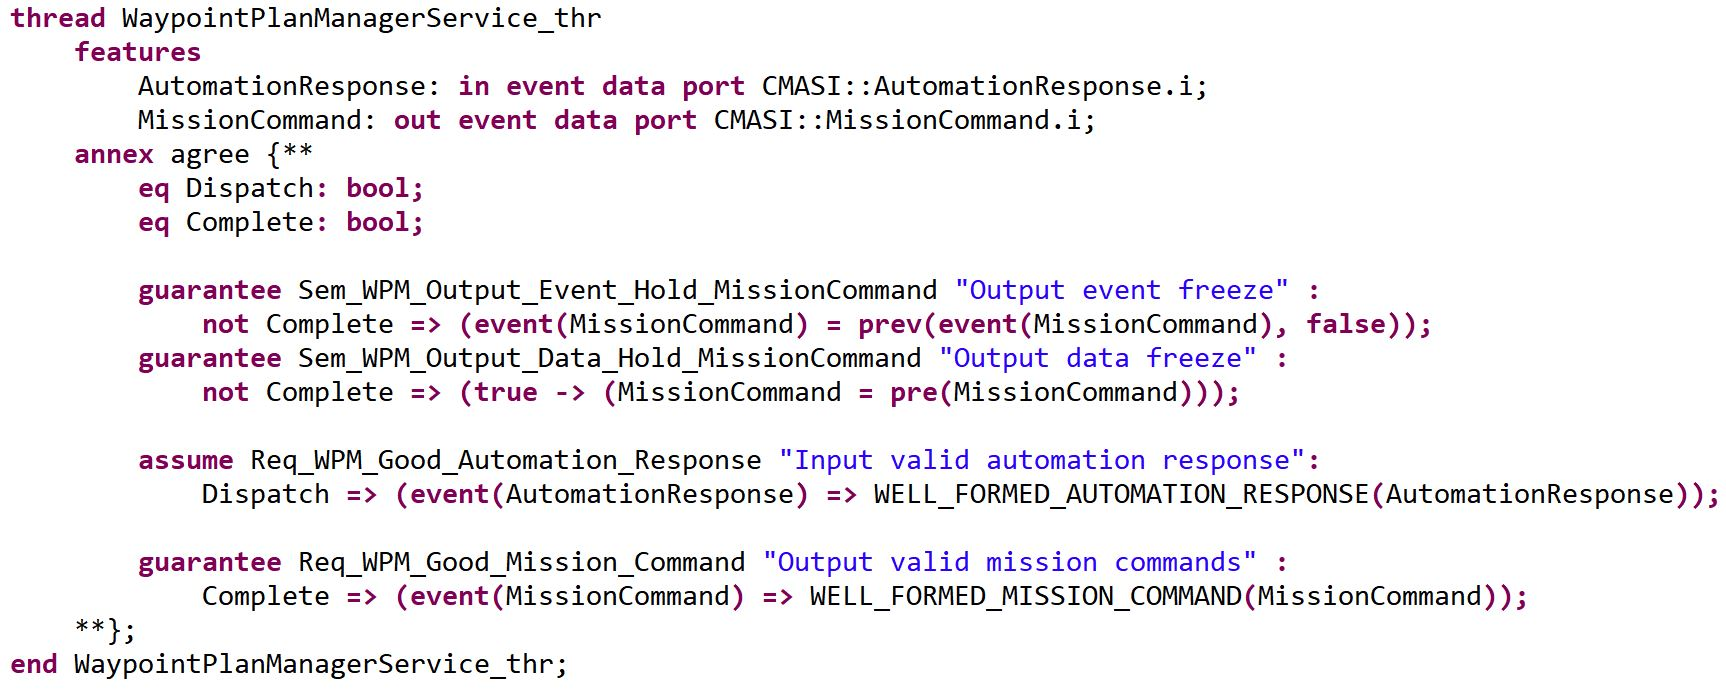
\includegraphics[width=130mm]{wpmAGREE3.jpg}
\caption{Direct Modelling Scheduling Semantics in AGREE\label{wpmAGREE}}
\end{figure}

At the system-level, we use a circular counter to model a cyclic schedule in AGREE. 
The counter updates at every instant. Once it reaches the limit, it resets to 1 at the next instant.
We set the limit to the period of the schedule. 
%The counter is a direct encoding of schedule $\phi$ defined previously.
Then based on the current count, a corresponding scheduling event is raised.
Figure \ref{schedule} shows an AGREE model of the schedule $(ABACD)$.

\begin{figure}[ht!]
\centering
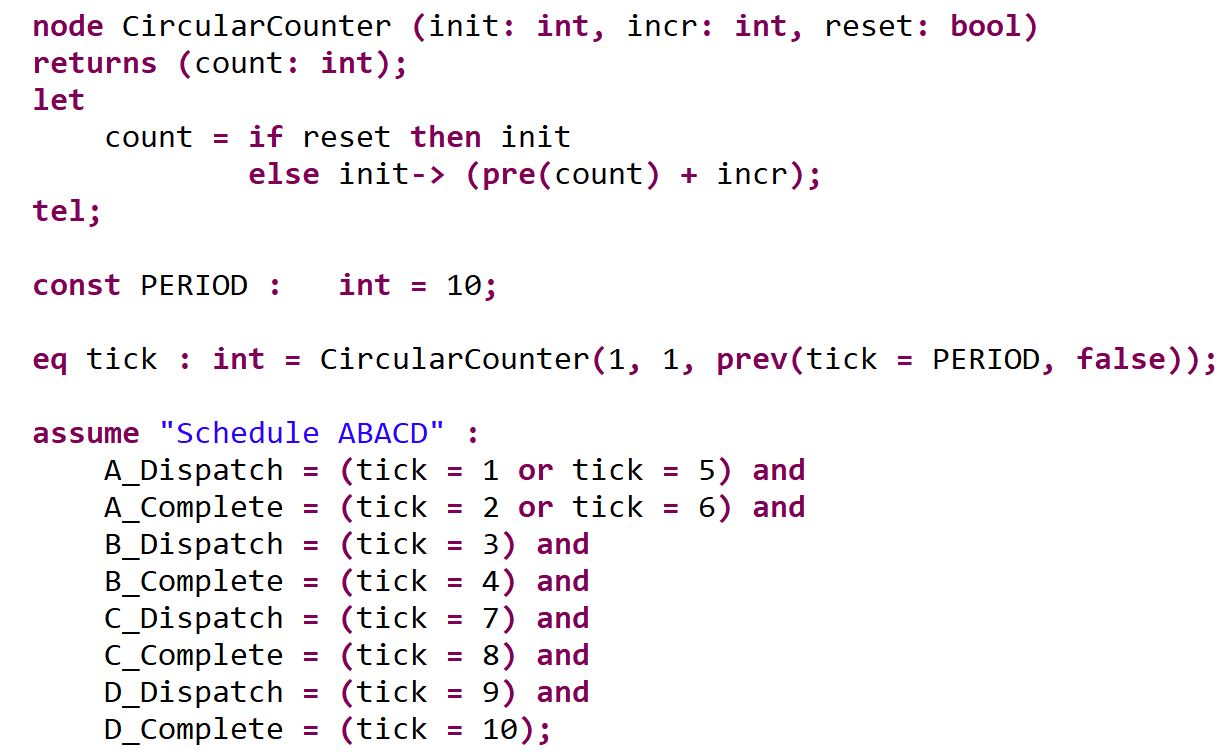
\includegraphics[width=80mm]{schedule.jpg}
\caption{A Model of Schedule in AGREE\label{schedule}}
\end{figure}

%An AGREE model of the schedule $(ABACD)^*$ used in the example is shown in code~\ref{schedule_model}

%\begin{lstlisting}[language=c,frame=single,caption=An AGREE model of a schedule,label=schedule_model]
%node CircularCounter (init: int, incr: int, reset: bool)	
%returns (count: int);
%let
%	count = if reset then init
%		else init-> (pre(count) + incr);
%tel;
%				
%eq tick : int = CircularCounter(1,1,prev(tick=10,false));
%
%assume "Schedule ABACD" :
%	A_dispatch = (tick = 1 or tick = 5) and
%	A_complete = (tick = 2 or tick = 6) and					
%	B_dispatch = (tick = 3) and	
%	B_complete = (tick = 4) and
%	C_dispatch = (tick = 7) and
%	C_complete = (tick = 8) and	
%	D_dispatch = (tick = 9) and
%	D_complete = (tick = 10);			
%\end{lstlisting}	



\section{LUSTRE Backend Model}
\label{lustre}
AGREE translates an AADL model and its annotated contracts into a dialect \cite{jkind} of the Lustre language, and then queries a user-selected model checker to perform the verification. The dialect includes an expression called \emph{condact}, which is similar to the activation condition in SCADE. It clocks a node call expression as follows: 
%%\begin{equation*}
%%condact (cond, node(node\_inputs, node\_outputs), init\_outputs)
%%\end{equation*}
$
condact (cond, node(node\_inputs, node\_outputs), init\_outputs)
$.
If the Boolean signal $cond$ is true, the clocked node $node$ is activated and updates its local and output signals. Otherwise, the node keeps the previous value of the local and output signals. Before the first activation, the node outputs values are set to \emph{init\_outputs}. %\emph{condact} is essential to model the scheduling semantics. 
We are aware that the standard Lustre language introduced similar temporal operators like \emph{when} and \emph{current}. We use \emph{condact} simply because it is supported by our default model checker JKind \cite{jkind}.

AGREE translates an AADL thread to a Lustre node in a \emph{constraint} style, in which the thread input and output ports are both mapped to the node input signals. Thus, the \emph{condact} expression does not automatically freeze the thread outputs. We add assertions to enforce the output freeze rule, and we use the thread \emph{complete} signal to clock the node. The \emph{complete} signal is triggered by the circular counter shown in Figure~\ref{schedule}. Figure~\ref{WPMlustre} shows an example of using \emph{condact} to model a scheduled AADL thread. 

\begin{figure}[t!]
\centering
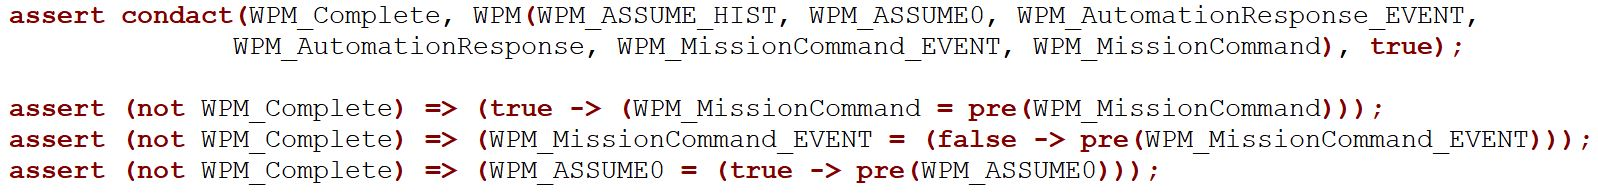
\includegraphics[width=120mm]{lustreAsync5.jpg}
\caption{A Lustre Model of a Scheduled AADL Thread \label{WPMlustre}}
\end{figure}

%\begin{figure}[ht!]
%\centering
%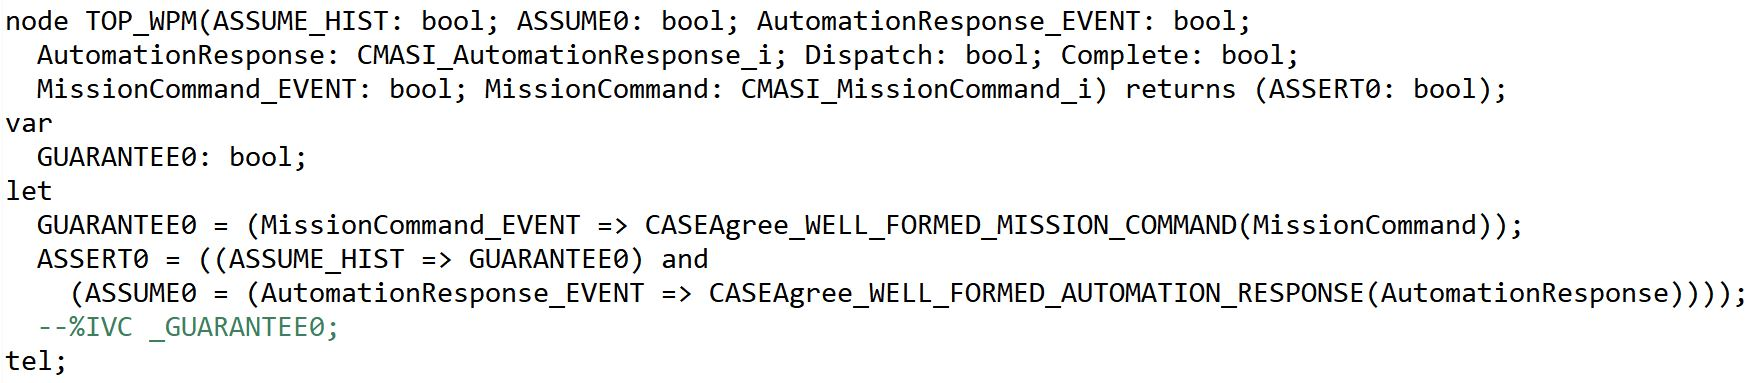
\includegraphics[width=130mm]{wpmLustre2.jpg}
%\caption{A Lustre Model of AADL Thread \label{WPMlustre}}
%\end{figure}
%
%\begin{figure}[ht!]
%\centering
%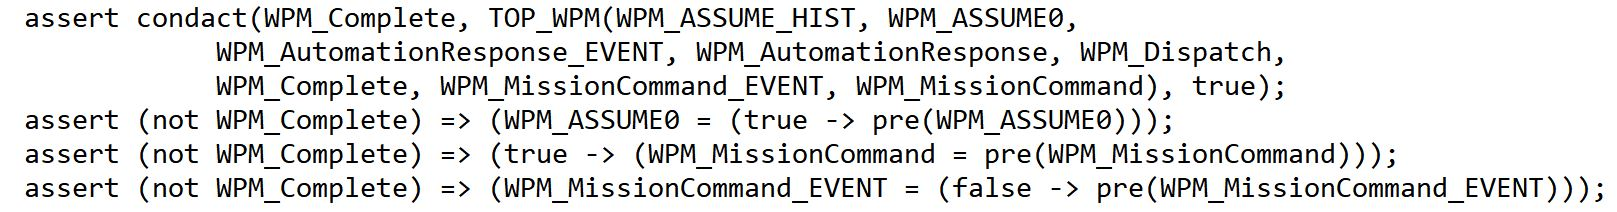
\includegraphics[width=130mm]{lustreAsync4.jpg}
%\caption{A Lustre Expression \emph{condact} Usage Example\label{lustreAsync}}
%\end{figure}
%
%\begin{figure}[ht!]
%\centering
%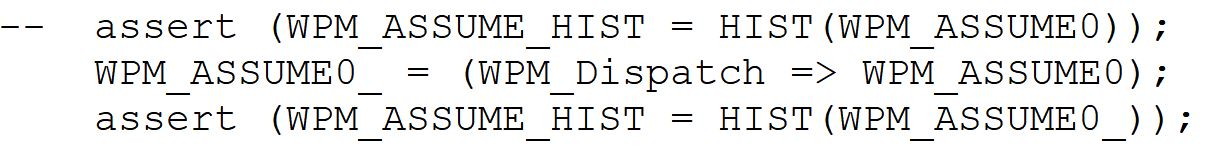
\includegraphics[width=80mm]{LustreAssume.jpg}
%\caption{An Example of Assumption Model in Lustre \label{lustreAsync}}
%\end{figure}

%\begin{figure}[ht!]
%\centering
%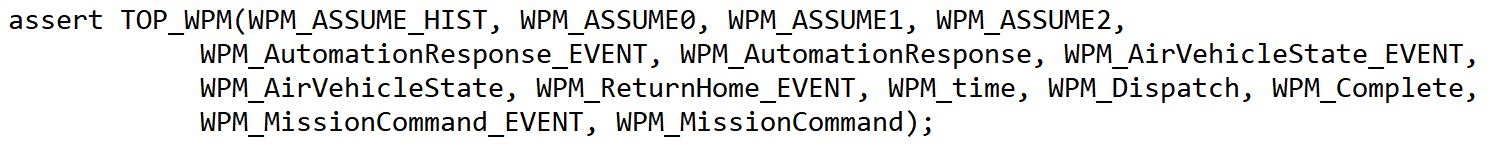
\includegraphics[width=120mm]{lustreSync2.jpg}
%\caption{An AADL Model Illustrating Motivation\label{lustreSync}}
%\end{figure}

%\begin{lstlisting}[language=c,frame=single,caption=An AGREE model of a schedule,label=schedule_model]
%  assert condact(WPM__Complete, _TOP__WPM(WPM____ASSUME__HIST, WPM____ASSUME0, WPM____ASSUME1, WPM____ASSUME2, 
%				WPM__AutomationResponse___EVENT_, WPM__AutomationResponse, WPM__AirVehicleState___EVENT_, WPM__AirVehicleState, 
%                WPM__ReturnHome___EVENT_, WPM__time, WPM__Dispatch, WPM__Complete, WPM__MissionCommand___EVENT_, WPM__MissionCommand), true);
%  assert (not WPM__Complete) => (WPM____ASSUME0 = (true -> pre(WPM____ASSUME0)));
%  assert (not WPM__Complete) => (WPM____ASSUME1 = (true -> pre(WPM____ASSUME1)));
%  assert (not WPM__Complete) => (WPM____ASSUME2 = (true -> pre(WPM____ASSUME2)));
%  assert (not WPM__Complete) => (true -> (WPM__MissionCommand = pre(WPM__MissionCommand)));
%  assert (not WPM__Complete) => (WPM__MissionCommand___EVENT_ = (false -> pre(WPM__MissionCommand___EVENT_)));
%\end{lstlisting}  
  


\section{Case Study}
\label{case-study}
Present phase2 simplified model


\section{Related Work}
\label{rw}
The AADL standard by iteself does not have a well-defined execution semantics. In order to formally verify an AADL model, it is often translated to a formal model \cite{AADL2TASM}, \cite{AADL2Sync}, \cite{AADL2TLA} \cite{AADS} \cite{AADL2BIP}. Then a formal method is applied to analyze the translated model.

Model checking of concurrent processes with specific schedules or scheduling constraints is a relatively new research area. Metzler et al. \cite{Metzler2020} use an iterative and incremental approach to prove safety properties of concurrent programs. It starts with a proof under a specific schedule, and then in each following iteration gradually relaxes the scheduling constraints. The iteration stops when all possible exections are explored or a counterexample is generated. Unlike our component model, their programs are ``white boxes'', allowing their schedule to interleave instructions between programs. However, in each iteration the model checking problem is 
still challenging. In this context, our compositional verification approach makes sense.

In \emph{aadl2sync} \cite{AADL2Sync}, the AADL behavior models are translated to synchronous programs mainly for simulation. It uses activation condition to model sporadic execution of software components, similar to our usage of \emph{condact}. However, the proposed framework focuses on simulating the timing behavior with the presence of clock drift. Meanwhile, we focus on the formal verification of system properties based on component contracts, which in general do not completely define component outputs.



\section{Conclusion and Future Work}
\label{conclusion}
{\bf Discussion.}
A schedule could also be specified as a set of precedence constraints, instead of an explicit sequence. However, this will potentially cause performance issues.

\section*{ACKNOWLEDGMENT}
This work was funded by DARPA contract HR00111890001. The
views, opinions and/or findings expressed are those of the author
and should not be interpreted as representing the official views or
policies of the Department of Defense or the U.S. Government.

We would like to thank John Hatcliff and Robby for many helpful discussions to clarify our understanding of the AADL semantics.
We also want to thank David Hardin and anonymous reviewers for their comments that greatly improved the paper.

%
% ---- Bibliography ----
%
% BibTeX users should specify bibliography style 'splncs04'.
% References will then be sorted and formatted in the correct style.
%
\bibliographystyle{splncs04}
\bibliography{paper}
%
\end{document}
